\pagestyle{empty}
\newgeometry{left=1.75cm,right=1.75cm,top=1.75cm,bottom=1.75cm}
%%%%%%%%%%%%%%%%%%%%%%%%%%%%%%%%%%%%%%%%%%%%%%%%%%%%%%%%%%%%%%%%%%%%%%%%%%%%%%%%
%%%%%%%%%%%%%%%%%%%%%%%%%%%%%%%%%%%%%%%%%%%%%%%%%%%%%%%%%%%%%%%%%%%%%%%%%%%%%%%%
%%%%%%%%%%%%%%%%%%%%%%%%%%%%%%%%%%%%%%%%%%%%%%%%%%%%%%%%%%%%%%%%%%%%%%%%%%%%%%%%
%%%%%%%%%%%%%%%%%%%%%%%%%%%%%%%%%%%%%%%%%%%%%%%%%%%%%%%%%%%%%%%%%%%%%%%%%%%%%%%%
\chapter[Analyse fréquentielle]
        {Analyse fréquentielle et représentation graphique\label{chap-repfreq}}
%%%%%%%%%%%%%%%%%%%%%%%%%%%%%%%%%%%%%%%%%%%%%%%%%%%%%%%%%%%%%%%%%%%%%%%%%%%%%%%%
%%%%%%%%%%%%%%%%%%%%%%%%%%%%%%%%%%%%%%%%%%%%%%%%%%%%%%%%%%%%%%%%%%%%%%%%%%%%%%%%
%%%%%%%%%%%%%%%%%%%%%%%%%%%%%%%%%%%%%%%%%%%%%%%%%%%%%%%%%%%%%%%%%%%%%%%%%%%%%%%%
%%%%%%%%%%%%%%%%%%%%%%%%%%%%%%%%%%%%%%%%%%%%%%%%%%%%%%%%%%%%%%%%%%%%%%%%%%%%%%%%
\minitoc
\newpage
%%%%%%%%%%%%%%%%%%%%%%%%%%%%%%%%%%%%%%%%%%%%%%%%%%%%%%%%%%%%%%%%%%%%%%%%%%%%%%%%
%%%%%%%%%%%%%%%%%%%%%%%%%%%%%%%%%%%%%%%%%%%%%%%%%%%%%%%%%%%%%%%%%%%%%%%%%%%%%%%%
%%%%%%%%%%%%%%%%%%%%%%%%%%%%%%%%%%%%%%%%%%%%%%%%%%%%%%%%%%%%%%%%%%%%%%%%%%%%%%%%
\section*{Réponse harmonique}
%%%%%%%%%%%%%%%%%%%%%%%%%%%%%%%%%%%%%%%%%%%%%%%%%%%%%%%%%%%%%%%%%%%%%%%%%%%%%%%%
%%%%%%%%%%%%%%%%%%%%%%%%%%%%%%%%%%%%%%%%%%%%%%%%%%%%%%%%%%%%%%%%%%%%%%%%%%%%%%%%
%%%%%%%%%%%%%%%%%%%%%%%%%%%%%%%%%%%%%%%%%%%%%%%%%%%%%%%%%%%%%%%%%%%%%%%%%%%%%%%%
%L'excitation d'un \SLCI~par une entrée sinuso\"idale donne lieu, en régime 
%permanent, à une réponse harmonique dépendant de la fréquence d'excitation. 
%Nous allons ici établir la forme de cette réponse.
Soit un \gls{slci}~défini par une fonction de transfert $H(p)$ auquel on 
applique une entrée sinuso\"idale $e(t)$ tel que :
\[
e(t)=E_0\sin\omega t 
\]
d'amplitude $E_0$ et de pulsation $\omega$\footnote{Strictement, $\omega$ est 
une pulsation en unité \si{\radian\per\second}, la fréquence associée étant 
$f=\omega/2\pi$, en \si{\per\second} ou \si{\hertz}. Cependant, par abus de 
langage, il est courant de se référer en terme de fréquence en parlant de la 
pulsation $\omega$. Nous prendrons cependant soin d'utiliser la bonne forme 
dans nos applications numériques.}. Dans le domaine de Laplace, la sortie $S(p)$
est de la forme :
\[
S(p)=H(p)E(p)
\]
où $E(p)$ est la transformée de Laplace d'un sinus (c.f ligne 23 du tableau de 
l'\cref{annexe-lap}), on obtient alors :
\[
S(p)=H(p)\dfrac{E_0\omega}{p^2+\omega^2}
\]
Les pôles de la fonction de transfert $H(p)$ donnent lieu au 
régime transitoire alors que les pôles de l'excitation donnent 
lieu au régime permanent. 
Les deux pôles de l'excitation sont $p_{1,2}=\pm\jw$. La forme factorisée 
s'écrit alors:
\[
S(p)=H(p)\dfrac{E_0\omega}{(p+\jw)(p-\jw)}
\]
En régime permanent, la décomposition de $S(p)$ en éléments simples s'écrit :
\[
S(p)=\dfrac{A}{p-\jw} + \dfrac{B}{p+\jw}
\]
où les coefficients s'obtiennent par évaluation :
%-------------------------------------------------------------------------------
\begin{align*}
    A&=(p-\jw)S(p)\bigg|_{p=\hphantom{-}\jw}=
       \dfrac{E_0\omega}{p+\jw}H(p)\bigg|_{p=\hphantom{-}\jw}=
       \hphantom{-}\dfrac{E_0}{2j}H(\jw)\\
    B&=(p+\jw)S(p)\bigg|_{p=-\jw}=
       \dfrac{E_0\omega}{p-\jw}H(p)\bigg|_{p=-\jw}=
       -\dfrac{E_0}{2j}H(-\jw)
\end{align*}
%-------------------------------------------------------------------------------
nous obtenons donc :
\[
S(p)=\dfrac{E_0}{2j}\left(\dfrac{H(\jw)}{p-\jw}-\dfrac{H(-\jw)}{p+\jw} \right)
\]
La transformée de Laplace inverse de la sortie $S(p)$ permet d'obtenir la 
réponse temporelle 
\[
s(t)=\dfrac{E_0}{2j}\left(H(\jw)e^{\jw t}-H(-\jw)e^{-\jw t}\right)
\]
En écrivant le nombre complexe $H(\jw)$ sous sa forme exponentielle 
(\Cref{annexe-NC}) :
%-------------------------------------------------------------------------------
\begin{align*}
    H(\jw)  &= |H(\jw)| e^{j\phi} \\
    H(-\jw) &= |H(\jw)| e^{-j\phi}
\end{align*}
%-------------------------------------------------------------------------------
où $|H(\jw)|$ et $\phi$ sont respectivement le module et l'argument du nombre
complexe $H(\jw)$ 
et où l'on montre de plus que $H(-\jw)$ est égale à son conjugué (c.-à-d. 
$H(-\jw)=\overline{H(\jw)}$).
%
%
% on peut montrer la symétrie conjuguée par le produit de convolution 
% MIT 6.003 Signals and Systems, Fall 2011   
% Video 9 . Frequency Response vers 36:39
%
%
La réponse temporelle peut alors s'écrire sous la forme 
%-------------------------------------------------------------------------------
\begin{align*}
s(t)=E_0|H(\jw)|\left(\dfrac{e^{j(\omega t+\phi)}
    -e^{-j(\omega t+\phi)}}{2j}\right)
\end{align*}
%-------------------------------------------------------------------------------
où l'on reconnaît la forme exponentielle de la fonction sinus qui nous permet
d'écrire :
%-------------------------------------------------------------------------------
\begin{bequation}[ams align]
    s(t)=E_0|H(\jw)|\sin{(\omega t+\phi)}\label{eq-rh}
\end{bequation}
%-------------------------------------------------------------------------------
Cette relation exprime que \textbf{l'excitation d'un {\protect{\gls{slci}}}
~par une entrée sinuso\"idale donne lieu, en régime permanent, à une réponse 
harmonique dépendant de la fréquence d'excitation dont le gain en amplitude et
la phase sont respectivement donné par le module et l'argument de la fonction
de transfert du système.}

\`A noter que $H(\jw)$ correspond au rapport de la sortie sur l'entrée,
ainsi le gain $|H(\jw)|$ et la phase peuvent être définits à partir de la 
sortie et de l'entrée du signal,
%-------------------------------------------------------------------------------
\begin{align*}
    H(\jw) &= \dfrac{S(\jw)}{E(\jw)} \\
    |H(\jw)|&= \dfrac{|S(\jw)|}{|E(\jw)|} \\
    \arg{H(\jw)}&=\arg{S(\jw)}-\arg{E(\jw)}
\end{align*}
%-------------------------------------------------------------------------------
Le gain $|H(\jw)|$ est une fonction réelle de $\omega$ de ce fait nous 
utiliserons par la suite $G(\omega)$ pour noter plus explicitement cette 
dépendance. La phase est également une fonction de la pulsation d'excitation, 
nous la noterons donc $\phi(\omega)$ par la suite.
%\newpage
\newgeometry{bottom=25mm,outer=60mm,marginparsep=3mm,marginparwidth=50mm}
\captionsetup{width=0.9\linewidth}
%%%%%%%%%%%%%%%%%%%%%%%%%%%%%%%%%%%%%%%%%%%%%%%%%%%%%%%%%%%%%%%%%%%%%%%%%%%%%%%%
%%%%%%%%%%%%%%%%%%%%%%%%%%%%%%%%%%%%%%%%%%%%%%%%%%%%%%%%%%%%%%%%%%%%%%%%%%%%%%%%
\subsection*{Réponse harmonique dans le domaine temporel}
%%%%%%%%%%%%%%%%%%%%%%%%%%%%%%%%%%%%%%%%%%%%%%%%%%%%%%%%%%%%%%%%%%%%%%%%%%%%%%%%
%%%%%%%%%%%%%%%%%%%%%%%%%%%%%%%%%%%%%%%%%%%%%%%%%%%%%%%%%%%%%%%%%%%%%%%%%%%%%%%%
\index{Système du premier ordre!réponse harmonique dans le domaine temporel}
Considérons un \gls{slci}~définit par une fonction de transfert $H(p)$ du 
premier ordre (\Cref{eq-ft1er}) de forme canonique:
\[
H(p)=\dfrac{1}{1+p}
\]
avec $K=$1, $\tau=\SI{1}{\second}$.

Comme nous venons de le montrer la réponse harmonique est complétement 
déterminée par la connaissance du module et de l'argument du nombre complexe
$H(\jw)$. Le module donnant accès au rapport du gain en amplitude de la sortie 
sur l'entrée et l'argument à la différence de phase entre la sortie et l'entrée.

Calculons donc ces deux quantités pour notre fonction de transfert du premier 
ordre:
%-------------------------------------------------------------------------------
\begin{align*}
    G(\omega)   &=|H(\jw)|               =\left|\dfrac{1}{1+\jtw}\right|\\
    \phi(\omega)&=\arg\left(H(\jw)\right)=-\arctan(\omega\tau)
\end{align*}
%-------------------------------------------------------------------------------
Le~\cref{tab-1ertemp} présente le module et l'argument pour quelques valeurs 
particulières de $\omega$ 
($\omega=0.1$, $1$ et $\SI{10}{\radian\per\second}$).
%-------------------------------------------------------------------------------
\begin{table}
    \ra{1.3}
    \centering
    \setlength{\ltmp}{2.0cm}
    \begin{tabular}{P{\ltmp}P{\ltmp}P{\ltmp}P{\ltmp}}
        \toprule
        $\omega\si{[\radian\per\second]}$&$\omega=0.1$&$\omega=1$&$\omega=10$\\
        \midrule
        $G(\omega)$         & 0.99       & 0.70       & 0.1                  \\
        \midrule
        $\phi(\omega)$      &-5.7\degreeSI &-45\degreeSI  &-84.3\degreeSI          \\
        \bottomrule
    \end{tabular}
\caption{Quelques valeurs particulières du gain et de la phase de la 
        fonction de transfert du premier ordre, pour $K=1$ et 
        $\tau=\SI{1}{\second}$\label{tab-1ertemp}.}
\end{table}
%-------------------------------------------------------------------------------
D'après ces valeurs, nous constatons que le rapport des amplitudes décroît et
que le déphasage augmente lorsque la pulsation de l'excitation augmente.

La~\cref{fig-repham} présente la forme des réponses temporelles de ce système 
pour les données calculées du gain et de la phase de la fonction de transfert 
considérée. Cette représentation graphique montre ses limites, en effet quand
est-il de toutes les autres valeurs de la pulsation ? 

Nous allons maintenant généraliser cette analyse sans pour autant avoir à 
tracer la réponse temporelle pour toutes les pulsations que l'on souhaite 
étudier.
%-------------------------------------------------------------------------------
\begin{marginfigure}[-20em]
    \centering
    \tikzsetnextfilename{repham_1-chap_repfreq-ext}
    \resizebox{\linewidth}{!}{\input{tikz/repham_1-chap_repfreq.tex}}
    \tikzsetnextfilename{repham_2-chap_repfreq-ext}
    \resizebox{\linewidth}{!}{\input{tikz/repham_2-chap_repfreq.tex}}
    \tikzsetnextfilename{repham_3-chap_repfreq-ext}
    \resizebox{\linewidth}{!}{\input{tikz/repham_3-chap_repfreq.tex}}
    \caption{Réponse harmonique (en régime permanent) (\Cref{eq-rh}) d'un 
             système du premier ordre pour différentes pulsations d'excitation 
             de la forme $e(t)=\sin{\omega t}$, (données du~\cref{tab-1ertemp}).
             Cette figure permet d'observer l'augmentation du déphasage et la 
             diminution de l'amplitude lorsque la fréquence d'excitations 
             augmente. (bleu) excitation $e(t)$ (rouge) sortie $s(t)$.
             \label{fig-repham}}
\end{marginfigure}
%-------------------------------------------------------------------------------
%%%%%%%%%%%%%%%%%%%%%%%%%%%%%%%%%%%%%%%%%%%%%%%%%%%%%%%%%%%%%%%%%%%%%%%%%%%%%%%%
%%%%%%%%%%%%%%%%%%%%%%%%%%%%%%%%%%%%%%%%%%%%%%%%%%%%%%%%%%%%%%%%%%%%%%%%%%%%%%%%
%\subsection{Réponse harmonique dans le domaine fréquentielle}
%%%%%%%%%%%%%%%%%%%%%%%%%%%%%%%%%%%%%%%%%%%%%%%%%%%%%%%%%%%%%%%%%%%%%%%%%%%%%%%%
%%%%%%%%%%%%%%%%%%%%%%%%%%%%%%%%%%%%%%%%%%%%%%%%%%%%%%%%%%%%%%%%%%%%%%%%%%%%%%%%
%\acpl
%\newpage
\clearpage
%%%%%%%%%%%%%%%%%%%%%%%%%%%%%%%%%%%%%%%%%%%%%%%%%%%%%%%%%%%%%%%%%%%%%%%%%%%%%%%%
%%%%%%%%%%%%%%%%%%%%%%%%%%%%%%%%%%%%%%%%%%%%%%%%%%%%%%%%%%%%%%%%%%%%%%%%%%%%%%%%
%%%%%%%%%%%%%%%%%%%%%%%%%%%%%%%%%%%%%%%%%%%%%%%%%%%%%%%%%%%%%%%%%%%%%%%%%%%%%%%%
\section*{Représentation graphique de 
la réponse harmonique}
%%%%%%%%%%%%%%%%%%%%%%%%%%%%%%%%%%%%%%%%%%%%%%%%%%%%%%%%%%%%%%%%%%%%%%%%%%%%%%%%
%%%%%%%%%%%%%%%%%%%%%%%%%%%%%%%%%%%%%%%%%%%%%%%%%%%%%%%%%%%%%%%%%%%%%%%%%%%%%%%%
%%%%%%%%%%%%%%%%%%%%%%%%%%%%%%%%%%%%%%%%%%%%%%%%%%%%%%%%%%%%%%%%%%%%%%%%%%%%%%%%
Comme nous venons de le voir, il est possible d'étudier
la réponse harmonique (en régime permanent) d'un \gls{slci}~dans le domaine 
temporel et observer la variation d'amplitude et du 
déphasage qui dépend de la pulsation d'excitation. Ces variations 
d'amplitude et de phase sont totalement déterminées par la 
connaissance du module et de l'argument du nombre complexe $H(\jw)$, 
c'est ce qui constitue l'analyse fréquentielle des \gls{slci}.

%%%%%%%%%%%%%%%%%%%%%%%%%%%%%%%%%%%%%%%%%%%%%%%%%%%%%%%%%%%%%%%%%%%%%%%%%%%%%%%%
%%%%%%%%%%%%%%%%%%%%%%%%%%%%%%%%%%%%%%%%%%%%%%%%%%%%%%%%%%%%%%%%%%%%%%%%%%%%%%%%
\subsection*{Diagramme de Bode}
%%%%%%%%%%%%%%%%%%%%%%%%%%%%%%%%%%%%%%%%%%%%%%%%%%%%%%%%%%%%%%%%%%%%%%%%%%%%%%%%
%%%%%%%%%%%%%%%%%%%%%%%%%%%%%%%%%%%%%%%%%%%%%%%%%%%%%%%%%%%%%%%%%%%%%%%%%%%%%%%%
\index{Diagramme! de Bode}
Le diagramme de Bode permet de représenter le comportement fréquentielle 
d'un système quelconque en fonction de la fréquence d'excitation en entrée. 
Il se compose de deux graphiques :
%-------------------------------------------------------------------------------
\begin{itemize}
    \item[i)] le tracé du gain en décibel en fonction de la pulsation $\omega$:
%-------------------------------------------------------------------------------
        \begin{bequation}[ams align] 
            G_{dB}(\omega)=20\log{G(\omega)}=20\log{|H(\jw)|} 
        \end{bequation}
%-------------------------------------------------------------------------------
    \item[ii)] le tracé de la phase en fonction de la pulsation $\omega$ :
%-------------------------------------------------------------------------------
        \begin{bequation}[ams align] 
            \phi(\omega)=\arg{H(\jw)}
        \end{bequation}
%-------------------------------------------------------------------------------
\end{itemize}
%-------------------------------------------------------------------------------
%-------------------------------------------------------------------------------
\begin{marginfigure}
    \centering
    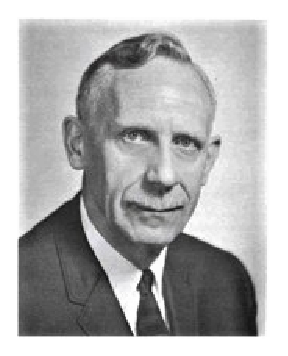
\includegraphics[width=0.9\linewidth]{HendrikBode.eps} 
    \caption*{\index{Bode, Hendrik}\textbf{Hendrik Wade Bode}
    (1905-1982), ingénieur, chercheur et inventeur américain.}
\end{marginfigure}
%-------------------------------------------------------------------------------
L'axe des pulsations étant généralement représenté par une échelle 
logarithmique pour permmettre la représentation de la réponse harmonique sur 
une large plage de valeurs en pulsation (\Cref{annexe-log}). Le calcul de la
phase passe lui par la détermination de l'argument principale 
(\Cref{annexe-NC}).
%-------------------------------------------------------------------------------
\begin{figure}[!h]
    \centering
    \tikzsetnextfilename{sche_bode-chap_repfreq-ext}
    \input{tikz/sche_bode-chap_repfreq.tex}
    \caption{Représentation schématique d'un diagramme de Bode. Le gain en 
             décibel et la phase associé à une fonction de transfert sont 
             représentés en fonction de la pulsation (à l'échelle log) sur 
             deux repères distincts.\label{fig-sche_bode}}
\end{figure}
%-------------------------------------------------------------------------------

La principale propriété du diagramme de Bode est de permettre de 
simplifier un grand nombre calcul. En effet, dans le cas par exemple où 
deux systèmes $H_1$ et $H_2$ sont mis en série,
\[
H(\jw)=H_1(\jw)H_2(\jw),
\]
Le diagramme de Bode de $H(\jw)$ est la somme de deux diagrammes indépendants:
\[
\mathrm{Bode}(total)=\mathrm{Bode}(1)+\mathrm{Bode}(2)
\]
\clearpage
\restoregeometry
\captionsetup{width=0.9\linewidth}
%%%%%%%%%%%%%%%%%%%%%%%%%%%%%%%%%%%%%%%%%%%%%%%%%%%%%%%%%%%%%%%%%%%%%%%%%%%%%%%%
%%%%%%%%%%%%%%%%%%%%%%%%%%%%%%%%%%%%%%%%%%%%%%%%%%%%%%%%%%%%%%%%%%%%%%%%%%%%%%%%
%%%%%%%%%%%%%%%%%%%%%%%%%%%%%%%%%%%%%%%%%%%%%%%%%%%%%%%%%%%%%%%%%%%%%%%%%%%%%%%%
\section*{Analyse fréquentielle des modèles usuels}
%%%%%%%%%%%%%%%%%%%%%%%%%%%%%%%%%%%%%%%%%%%%%%%%%%%%%%%%%%%%%%%%%%%%%%%%%%%%%%%%
%%%%%%%%%%%%%%%%%%%%%%%%%%%%%%%%%%%%%%%%%%%%%%%%%%%%%%%%%%%%%%%%%%%%%%%%%%%%%%%%
%%%%%%%%%%%%%%%%%%%%%%%%%%%%%%%%%%%%%%%%%%%%%%%%%%%%%%%%%%%%%%%%%%%%%%%%%%%%%%%%
%%%%%%%%%%%%%%%%%%%%%%%%%%%%%%%%%%%%%%%%%%%%%%%%%%%%%%%%%%%%%%%%%%%%%%%%%%%%%%%%
%%%%%%%%%%%%%%%%%%%%%%%%%%%%%%%%%%%%%%%%%%%%%%%%%%%%%%%%%%%%%%%%%%%%%%%%%%%%%%%%
\subsection*{Diagrammes de Bode}
%%%%%%%%%%%%%%%%%%%%%%%%%%%%%%%%%%%%%%%%%%%%%%%%%%%%%%%%%%%%%%%%%%%%%%%%%%%%%%%%
%%%%%%%%%%%%%%%%%%%%%%%%%%%%%%%%%%%%%%%%%%%%%%%%%%%%%%%%%%%%%%%%%%%%%%%%%%%%%%%%
%%%%%%%%%%%%%%%%%%%%%%%%%%%%%%%%%%%%%%%%%%%%%%%%%%%%%%%%%%%%%%%%%%%%%%%%%%%%%%%%
\subsubsection*{Méthodologie générale}
%%%%%%%%%%%%%%%%%%%%%%%%%%%%%%%%%%%%%%%%%%%%%%%%%%%%%%%%%%%%%%%%%%%%%%%%%%%%%%%%
Pour chacun des modèles usuels, à savoir : un gain pur, un intégrateur pur,
un dérivateur pur, un retard pur, un système du premier ordre et du second 
ordre, nous allons déterminer les diagrammes de Bode dits asymptotiques 
et réels. Le diagramme réel est la représentation exacte des fonctions du gain
en décibel et de la phase en fonction de la pulsation d'entrée de 
la sollicitation. Le diagramme asymptotique permet de caractériser 
qualitativement l'effet du modèle usuel sur le diagramme de Bode. 
Dans la pratique, on ne s'interresse qu'aux limites aux basses et hautes 
fréquences. Nous pourrons vérifier que cette approximation asymptotiques est une
approximation pour la fonction du gain.

Pour résumer, nous appliquerons la procédure suivante à chacun des modèles 
usuels :
%-------------------------------------------------------------------------------
\begin{itemize}
    \item[i)] Définir la fonction de transfert complexe $H(\jw)$ à partir de la 
          fonction de transfert $H(p)$ du modèle en question pour $p=\jw$.
    \item[ii)] \'Etablir la fonction du gain $G(\omega)$ à partir du 
          module de $H(\jw)$.
    \item[iii)] Déterminer le gain en décibel $G_{\si{\dB}}$ tel que 
        $G_{\si{\dB}}=20\log{G(\omega)}$.
    \item[iv)] \'Etablir la fonction de la phase $\phi(\omega)$ à partir de 
        l'argument principale de $H(\jw)$.
        \footnote{L'argument principale est l'argument d'un nombre complexe 
        dans $[-\pi,\pi]$. On se raportera à l'\Cref{annexe-NC} pour plus 
        de détails.}
    \item[v)] Si les fonctions $G(\omega)$ et $\phi(\omega)$ ne sont pas de 
          simples constantes, réalisér une étude
          asymptotique pour $\omega\rightarrow 0$ et 
          $\omega\rightarrow +\infty$.
    \item[vi)] Tracer le diagramme de Bode \textbf{réel} et le diagramme 
          de Bode \textbf{asymptotique} sur un graphe semi-logarithmique.
\end{itemize}
%-------------------------------------------------------------------------------
%%%%%%%%%%%%%%%%%%%%%%%%%%%%%%%%%%%%%%%%%%%%%%%%%%%%%%%%%%%%%%%%%%%%%%%%%%%%%%%%
\subsubsection*{Diagramme de Bode d'un système du premier ordre}
%%%%%%%%%%%%%%%%%%%%%%%%%%%%%%%%%%%%%%%%%%%%%%%%%%%%%%%%%%%%%%%%%%%%%%%%%%%%%%%%
\index{Système du premier ordre!diagramme de Bode}
Un système du premier ordre présente une fonction de transfert de la forme:
%-------------------------------------------------------------------------------
\begin{align}
H(\jw)=\dfrac{K}{1+j\tau\omega }\label{eq-1er_ftjw}
\end{align}
%-------------------------------------------------------------------------------
Le module de cette fonction de transfert $G(\omega) =|H(\jw)|$ s'écrit :
\[
    G(\omega)=\dfrac{K}{\sqrt{1+\tau^2\omega^2}}
\]
Le gain en dB s'obtient alors par :
%-------------------------------------------------------------------------------
\begin{bequation}[ams align]
    G_{dB}(\omega)=20\log{K}-20\log{\sqrt{1+\tau^2\omega^2}}\label{eq-gain_1er}
\end{bequation}
%-------------------------------------------------------------------------------
et la phase est simplement donné par la fonction tangente réciproque:
%-------------------------------------------------------------------------------
\begin{bequation}[ams align]
    \phi(\omega)=\arg{H(\jw)}=-\arctan{(\tau\omega)}\label{eq-phase_1er} 
\end{bequation}
%-------------------------------------------------------------------------------
Ce sont ces deux fonctions de la fréquence que nous traçons sur un diagramme
de Bode. Elles sont représentés sur les~\cref{fig-bode_1er_1,fig-bode_1er_2}, 
pour respectivement différentes valeurs du gain statique $K$ et du temps 
caractéristique $\tau$.
\newline
Il est cependant recommandé de déterminer les asymptotes 
de ces deux fonctions à basse et haute fréquence. 
Pour celà, nous introduisons une \textbf{fréquence de cassure} 
$\omega_c=\dfrac{1}{\tau}$ qui délimite ces deux domaines.
\`A cette fréquence, le gain en décibel est de $G_{dB}(\omega_c)=20\log{K}-3$ 
et la phase $\phi(\omega)=\arctan{(1)}=\dfrac{\pi}{4}$.
Le gain de -3dB est la valeur approximative de $20\log{\sqrt{2}}$, communément
utilisée pour définir la \textbf{fréquence de coupure}.

\`A basse fréquence, c'est à dire lorsque $\tau\omega\ll1$ ou 
encore $\omega\ll\omega_0$, le gain et la phase se comporte comme, 
%-------------------------------------------------------------------------------
\begin{bequation}[ams align*]
    G_{dB}(\omega)&\sim20\log{K} \\
    \phi(\omega)&\sim0\degreeSI.
\end{bequation} 
%-------------------------------------------------------------------------------
\`A haute fréquence, c'est à dire lorsque $\tau\omega\gg1$ ou 
encore $\omega\gg\omega_0$, le gain et la phase se comporte comme,
%-------------------------------------------------------------------------------
\begin{bequation}[ams align*]
    G_{dB}(\omega)&\sim20\log{K}-20\log{\frac{\omega}{\omega_0}} \\
    \phi(\omega)&\sim-\dfrac{\pi}{2}.
\end{bequation} 
%-------------------------------------------------------------------------------
La~\cref{fig-bode_1er_3} présente sur un même diagramme de Bode, les courbes 
réels et les courbes asymptotiques.
%-------------------------------------------------------------------------------
\begin{figure}[!t]
    \centering
    \tikzsetnextfilename{bode_1er_1-chap_repfreq-ext}
    \input{tikz/bode_1er_1-chap_repfreq.tex}

    \tikzsetnextfilename{bode_1er_2-chap_repfreq-ext}
    \input{tikz/bode_1er_2-chap_repfreq.tex}
    \caption{Diagramme de Bode d'un système du premier ordre 
             (\Cref{eq-1er_ftjw}) avec (noir) $K=0.1$ (bleu) $K=1$ et 
             (rouge) $K=10$. L'effet du gain $K$ est de décaler verticalement 
             la courbe de gain.\label{fig-bode_1er_1}}
\end{figure}
%-------------------------------------------------------------------------------
%-------------------------------------------------------------------------------
\begin{figure}[!b]
    \centering
    \tikzsetnextfilename{bode_1er_3-chap_repfreq-ext}
    \input{tikz/bode_1er_3-chap_repfreq.tex}

    \tikzsetnextfilename{bode_1er_4-chap_repfreq-ext}
    \input{tikz/bode_1er_4-chap_repfreq.tex}
    \caption{Diagramme de Bode d'un système du premier ordre 
             (\Cref{eq-1er_ftjw}) avec (noir) $\tau=10$ (bleu) $\tau=1$ et 
             (rouge) $\tau=0.1$. L'effet du temps caractéristique $\tau$ est 
             de décaler horizontalement la courbe de phase.
             \label{fig-bode_1er_2}}
\end{figure}
%-------------------------------------------------------------------------------
\afterpage{\clearpage}
%-------------------------------------------------------------------------------
\begin{figure}[!t]
\centering
\tikzsetnextfilename{bode_1er_5-chap_repfreq-ext}
\begin{tikzpicture}[trim axis left]
\begin{axis}[
    ticklabel style = {font=\footnotesize},
    width=0.9\textwidth,
    height=0.22\textheight,
    ylabel={Gain (dB)},
    xtick={1e-1,1,1e1}, 
    ytick={-10,-8,-6,-4,-2,0,2}, 
    xticklabels={$10^{-1}$,$10^{0}$,$10^{1}$},
    yticklabels={-10,-8,-6,-4,-2,0,2}, 
    xmode=log,ymode=normal,
    xmin=1e-1, xmax=1e1,
    ymin=-10, ymax=3,
    grid=both,
    major grid style={black!40}
]
    \addplot[ultra thick,col1,domain=1e-3:1e3, samples=101] 
    {-20*log10(sqrt(1+x*x))};
    \addplot[line width=2pt,col4,dashed,domain=1e-1:1e0, samples=101] {0};
    \addplot[line width=2pt,col4,dashed,domain=1e0:1e1, samples=101] 
    {-20*log10(x)};
\end{axis}
\end{tikzpicture}


\tikzsetnextfilename{bode_1er_6-chap_repfreq-ext}
\begin{tikzpicture}[trim axis left]
\begin{axis}[
    ticklabel style = {font=\footnotesize},
    width=0.9\textwidth,
    height=0.22\textheight,
    xlabel={Pulsation (rad/s)},
    ylabel={Phase (deg)},
    xtick={1e-1,1,1e1}, 
    ytick={-90,-45,0}, 
    yticklabels={-90,-45,0},
    xticklabels={$10^{-1}$,$10^{0}$,$10^{1}$},
    xmode=log,ymode=normal,
    xmin=1e-1, xmax=1e1,
    ymin=-90, ymax=0,
    grid=both,
    major grid style={black!40}
]
    \addplot[ultra thick,col1,domain=1e-3:1e3, samples=101] {-atan2(x,1)};
    \addplot[line width=2pt,col4,dashed,domain=1e-1:1e0,samples=101] {0};
    \addplot[line width=2pt,col4,dashed,domain=1e0:1e1,samples=101] {-90};
    \draw[line width=2pt,col4,dashed] (axis cs:1,0) -- (axis cs:1,-90);
\end{axis}
\end{tikzpicture}

\caption{Diagramme de Bode d'un système du premier ordre 
         (\Cref{eq-1er_ftjw}) (c.-à-d. $K=1$, $\tau=1$ et $\omega_c=1$) avec 
         (bleu) le diagramme réel et (rouge) le diagramme asymptotique. On 
         vérifie que les valeurs asymptotiques sont de bonnes approximations 
         à basse et haute fréquence. Il est également possible de lire un 
         gain de \SI{-3}{\dB} et une phase de -45\degreeSI à la fréquence 
         de coupure.\label{fig-bode_1er_3}}
\end{figure}
%-------------------------------------------------------------------------------
%%%%%%%%%%%%%%%%%%%%%%%%%%%%%%%%%%%%%%%%%%%%%%%%%%%%%%%%%%%%%%%%%%%%%%%%%%%%%%%%
\subsubsection*{Diagramme de Bode de deux systèmes du premier ordre en série }
%%%%%%%%%%%%%%%%%%%%%%%%%%%%%%%%%%%%%%%%%%%%%%%%%%%%%%%%%%%%%%%%%%%%%%%%%%%%%%%%
La fonction de transfert globale de deux systèmes du premier ordre en série 
s'écrit:
%-------------------------------------------------------------------------------
\begin{align}
    H(\jw)=\dfrac{K_1K_2}{(1+j\tau_1\omega)(1+j\tau_2\omega)}
    \label{eq-1er_serie}
\end{align}
%-------------------------------------------------------------------------------
On utilise la propriété du logarithme pour écrire le gain globale 
$G_{dB}(\omega)$ comme une somme de gain de deux systèmes du premier ordre, 
soit
\[
G_{dB}(\omega) = G_{dB1}(\omega) + G_{dB2}(\omega)
\]
De même pour la phase:
\[
\phi(\omega)= \phi_1(\omega) + \phi_2(\omega)
\]
En reprenant les~\cref{eq-gain_1er,eq-phase_1er} on établit facilement que,
%-------------------------------------------------------------------------------
\begin{bequation}[ams align*]
    G_{dB}(\omega) = 20\log{K_1K_2}-20\log{\sqrt{1+\tau_1^2\omega^2}}
                    -20\log{\sqrt{1+\tau_2^2\omega^2}}
\end{bequation}
%-------------------------------------------------------------------------------
et
%-------------------------------------------------------------------------------
\begin{bequation}[ams align*]
    \phi(\omega)=-\arctan{\tau_1\omega}-\arctan{\tau_2\omega}
\end{bequation}
%-------------------------------------------------------------------------------
L'étude asymptotique se fait en considérant deux fréquences de coupures 
$\omega_{c1}=\frac{1}{\tau_1}$ et $\omega_{c2}=\frac{1}{\tau_2}$.
Supposons d'abord, sans perte de généralité, que $\omega_{c2}>\omega_{c1}$ et 
considérons 
les trois domaines de fréquence ainsi définits selon que 
$\omega\ll\omega_{c1}$, $\omega_{c1}<\omega<\omega_{c1}$ ou 
$\omega\gg\omega_{c2}$
%%%%%%%%%%%%%%%%%%%%%%%%%%%%%%%%%%%%%%%%%%%%%%%%%%%%%%%%%%%%%%%%%%%%%%%%%%%%%%%%
\paragraph{Pour $\omega\ll\omega_{c1}$}
%%%%%%%%%%%%%%%%%%%%%%%%%%%%%%%%%%%%%%%%%%%%%%%%%%%%%%%%%%%%%%%%%%%%%%%%%%%%%%%%
%-------------------------------------------------------------------------------
\begin{bequation}[ams align*]
    G_{dB}(\omega)&\sim20\log{K_1K_2}\\
      \phi(\omega)&\sim0\degreeSI
\end{bequation}
%-------------------------------------------------------------------------------
%%%%%%%%%%%%%%%%%%%%%%%%%%%%%%%%%%%%%%%%%%%%%%%%%%%%%%%%%%%%%%%%%%%%%%%%%%%%%%%%
\paragraph{Pour $\omega_{c1}<\omega<\omega_{c1}$}
%%%%%%%%%%%%%%%%%%%%%%%%%%%%%%%%%%%%%%%%%%%%%%%%%%%%%%%%%%%%%%%%%%%%%%%%%%%%%%%%
%-------------------------------------------------------------------------------
\begin{bequation}[ams align*]
    G_{dB}(\omega)&\sim20\log{K_1K_2}-20\log{\dfrac{\omega}
                                        {\omega_{c1}\omega_{c2}}}\\
    \phi(\omega)&\sim-90\degreeSI
\end{bequation}
%-------------------------------------------------------------------------------
%%%%%%%%%%%%%%%%%%%%%%%%%%%%%%%%%%%%%%%%%%%%%%%%%%%%%%%%%%%%%%%%%%%%%%%%%%%%%%%%
\paragraph{Pour $\omega\gg\omega_{c2}$}
%%%%%%%%%%%%%%%%%%%%%%%%%%%%%%%%%%%%%%%%%%%%%%%%%%%%%%%%%%%%%%%%%%%%%%%%%%%%%%%%
%-------------------------------------------------------------------------------
\begin{bequation}[ams align*]
    G_{dB}(\omega)&\sim20\log{K_1K_2}-40\log{\dfrac{\omega}
                                        {\omega_{c1}\omega_{c2}}}\\
    \phi(\omega)&\sim-180\degreeSI
\end{bequation}
%-------------------------------------------------------------------------------
La~\cref{fig-bode_1er_serie} présente le diagramme de Bode réel et 
asymptotique de deux systèmes du premier ordre en cascade. On remarquera 
que l'approximation asymptotique est suffisante pour décrire le gain de ce 
genre de système. En marquant la discontinuité dans le graphe de la phase, 
on distingue plus facilement les différentes zones et les changements de 
pente du gain. Pour la phase, il suffit de déterminer sa valeur pour 
quelques valeurs particulières de la pulsation. 

Comme nous l'avons déjà rencontré, l'étude de deux systèmes du premier 
ordre en série correspond à l'étude d'un système du second ordre en 
régime apériodique.
%-------------------------------------------------------------------------------
\begin{figure}[!t]
    \centering
    \tikzsetnextfilename{bode_1er_serie_2nd_1-chap_repfreq-ext}
    \begin{tikzpicture}[trim axis left]
\begin{axis}[
    ticklabel style = {font=\footnotesize},
    width=0.9\textwidth,
    height=0.25\textheight,
    ylabel={Gain (dB)},
    xtick={1e-3,1e-2,1e-1,1,1e1,1e2,1e3}, 
    ytick={-80,-60,-40,-20,0,20,40,60}, 
    xticklabels={$10^{-3}$,$10^{-2}$,$10^{-1}$,
                 $10^{0}$,$10^{1}$,$10^{2}$,$10^{3}$},
    yticklabels={-80,-60,-40,-20,0,20,40,60}, 
    xmode=log,ymode=normal,
    xmin=1e-3, xmax=1e3,
    ymin=-120, ymax=20,
    grid=both,
    major grid style={black!40}
]
    \addplot[ultra thick, col1,domain=1e-3:1e3, samples=101]
    {-20*log10(sqrt(1+100*x*x))-20*log10(sqrt(1+0.01*x*x))}; 
    \addplot[line width=2pt,col4,dashed,domain=1e-3:1e-1, samples=101]{0};
    \addplot[line width=2pt,col4,dashed,domain=1e-1:1e1, samples=101]
    {-20*log10(x/0.1)};
    \addplot[line width=2pt,col4,dashed,domain=1e1:1e3, samples=101]
    {-20*log10(x/0.1)-20*log10(x/10)};
    \node[right,xshift=1em,yshift=-0.1em] at (axis cs:0.1,-70)
    {{\large \textbf{-20dB/décade}}};
    \node[right,xshift=1em,yshift=-0.1em] at (axis cs:10,-10)
    {{\large \textbf{-40dB/décade}}};
\end{axis}
\end{tikzpicture}


    \tikzsetnextfilename{bode_1er_serie_2nd_2-chap_repfreq-ext}
    \input{tikz/bode_1er_serie_2nd_2-chap_repfreq.tex}
    \caption{Diagramme de Bode de systèmes du premier ordre en série 
    (\Cref{eq-1er_serie}) avec $\tau_1=10$ et $\tau_2=0.1$ (bleu) le 
    diagramme réel et (rouge) le diagramme asymptotique.
    \label{fig-bode_1er_serie}}
\end{figure}
%-------------------------------------------------------------------------------
%\newpage
%%%%%%%%%%%%%%%%%%%%%%%%%%%%%%%%%%%%%%%%%%%%%%%%%%%%%%%%%%%%%%%%%%%%%%%%%%%%%%%%
\subsubsection*{Diagramme de Bode d'un système second d'ordre}
%%%%%%%%%%%%%%%%%%%%%%%%%%%%%%%%%%%%%%%%%%%%%%%%%%%%%%%%%%%%%%%%%%%%%%%%%%%%%%%%
\index{Système du second ordre!diagramme de Bode}
La fonction de transfert d'un système du second ordre (\Cref{eq-2nd_ft}) 
est donnée par :
%-------------------------------------------------------------------------------
\begin{align}
    H(\jw)=\dfrac{K\omega^2_0}{(\omega^2_0-\omega^2)+j2\xi\omega_0\omega}
    \label{eq-2nd_ftjw}
\end{align}
%-------------------------------------------------------------------------------
Le gain s'obtient en calculant le module de ce nombre complexe :
\[
    G(\omega)=\dfrac{K\omega^2_0}{\sqrt{(\omega^2_0-\omega^2)^2
         +(2\xi\omega_0\omega)^2}}
\]
Le gain en décibel s'écrit alors :
%-------------------------------------------------------------------------------
\begin{bequation}[ams align*]
    G_{db}(\omega)=20\log{K\omega_0^2}-20\log{\sqrt{(\omega^2_0-\omega^2)^2
                                               +(2\xi\omega_0\omega)^2}}
\end{bequation}
%-------------------------------------------------------------------------------
et la phase par l'argument princiale:
%-------------------------------------------------------------------------------
\begin{bequation}[ams align*]
    \phi(\omega)=
    \begin{cases}
    -\arctan{\left(\dfrac{2\xi\omega_0\omega}{\omega_0^2-\omega^2}\right)}     
        &\,\,\,\,\text{si $\omega^2<\omega^2_0$}\\
    -\arctan{\left(\dfrac{2\xi\omega_0\omega}{\omega_0^2-\omega^2}\right)}+\pi 
        &\,\,\,\,\text{si $\omega^2>\omega^2_0$}\\
    -\dfrac{\pi}{2}                                                            
    &\,\,\,\,\text{si $\omega^2=\omega^2_0$}
    \end{cases}
\end{bequation}
%-------------------------------------------------------------------------------
Comme précédemment, il est recommandé d'étudier les valeurs asymptotiques 
du gain et de la phase.
%%%%%%%%%%%%%%%%%%%%%%%%%%%%%%%%%%%%%%%%%%%%%%%%%%%%%%%%%%%%%%%%%%%%%%%%%%%%%%%%
\paragraph{Pour $\omega \ll\omega_0$}
%%%%%%%%%%%%%%%%%%%%%%%%%%%%%%%%%%%%%%%%%%%%%%%%%%%%%%%%%%%%%%%%%%%%%%%%%%%%%%%%
%-------------------------------------------------------------------------------
\begin{bequation}[ams align*]
    G_{dB}(\omega)&\sim20\log{K}\\
    \phi(\omega)&\sim0\degreeSI
\end{bequation}
%-------------------------------------------------------------------------------
%%%%%%%%%%%%%%%%%%%%%%%%%%%%%%%%%%%%%%%%%%%%%%%%%%%%%%%%%%%%%%%%%%%%%%%%%%%%%%%%
\paragraph{Pour $\omega \gg\omega_0$}
%%%%%%%%%%%%%%%%%%%%%%%%%%%%%%%%%%%%%%%%%%%%%%%%%%%%%%%%%%%%%%%%%%%%%%%%%%%%%%%%
%-------------------------------------------------------------------------------
\begin{bequation}[ams align*]
G_{dB}(\omega)&\sim20\log{K\omega^2_0}-40\log\omega\\
    \phi(\omega)&\sim-180\degreeSI
\end{bequation}
%-------------------------------------------------------------------------------
La~\cref{fig-bode_2nd_1} présente le diagramme de Bode associé à ces deux 
fonctions pour $\xi=1$, ainsi que le diagramme de Bode asymptotique. 
La~\cref{fig-bode_2nd_2} présente l'effet du taux d'amortissement $\xi$ sur 
le diagramme de Bode. Il est possible d'observer une augmentation de la valeur 
maximum du gain proche de la fréquence de coupure.
C'est ce phénomène de résonance que nous allons discuter dans la 
prochaine partie.
%-------------------------------------------------------------------------------
\begin{figure}[!t]
    \centering
    \tikzsetnextfilename{bode_2nd_1-chap_repfreq-ext}
    \begin{tikzpicture}[trim axis left]
\begin{axis}[
    ticklabel style = {font=\footnotesize},
    width=0.9\textwidth,
    height=0.22\textheight,
    ylabel={Gain (dB)},
    xtick={1e-3,1e-2,1e-1,1,1e1,1e2,1e3}, 
    ytick={-120,-100,-80,-60,-40,-20,0,20,40,60}, 
    xticklabels={$10^{-3}$,$10^{-2}$,$10^{-1}$,
                 $10^{0}$,$10^{1}$,$10^{2}$,$10^{3}$},
    yticklabels={-120,-100,-80,-60,-40,-20,0,20,40,60}, 
    xmode=log,ymode=normal,
    xmin=1e-3, xmax=1e3,
    ymin=-100, ymax=20,
    grid=both,
    major grid style={black!40},
    cycle list name=color list,
]
    \addplot[signalr,dashed,domain=1e-3:1e0]{0};
    \addplot[signalr,dashed,domain=1e0:1e3] 
    {-40*log10(x)};
    \foreach \a in {1.0}
        \addplot[signalb,domain=1e-3:1e3] 
        {-20*log10(sqrt( (1-x*x)^2 +(2*\a*x)^2 )  )}; 
\end{axis}
\end{tikzpicture}


    \tikzsetnextfilename{bode_2nd_2-chap_repfreq-ext}
    \begin{tikzpicture}[trim axis left]
\begin{axis}[
    legend style={draw=none},    
    legend pos=outer north east, 
    ticklabel style = {font=\footnotesize},
    width=0.9\textwidth,
    height=0.22\textheight,
    xlabel={Pulsation (rad/s)},
    ylabel={Phase (deg)},
    xtick={1e-3,1e-2,1e-1,1,1e1,1e2,1e3}, 
    ytick={-180,-135,-90,-45,0}, 
    yticklabels={-180,-135,-90,-45,0},
    xticklabels={$10^{-3}$,$10^{-2}$,$10^{-1}$,
                 $10^{0}$,$10^{1}$,$10^{2}$,$10^{3}$},
    xmode=log,ymode=normal,
    xmin=1e-3, xmax=1e3,
    ymin=-180, ymax=0,
    grid=both,
    major grid style={black!40},
    cycle list name=color list,
]
    \addplot[signalr,dashed,domain=1e-3:1e0] {0};
    \addplot[signalr,dashed,domain=1e0:1e3] {-180};
    \draw[signalr,dashed] (axis cs:1,0) -- (axis cs:1,-180);
    \foreach \a in {1.0}
        \addplot+[signalb,domain=1e-3:1e3] 
        {-atan2(2*\a*x,(1-x*x))}; 
\end{axis}
\end{tikzpicture}

    \caption{Diagramme de Bode d'une fonction de transfert second ordre 
    (\Cref{eq-2nd_ftjw}) avec $K=1$, $\omega_0=1$ et $\xi=1$
    \label{fig-bode_2nd_1}}
\end{figure}
%-------------------------------------------------------------------------------
\begin{figure}[!t]
    \centering
    \tikzsetnextfilename{bode_2nd_3-chap_repfreq-ext}
    \newcommand{\LHS}[2][1.5em]{\hspace{#1}\mathllap{#2}}
\begin{tikzpicture}
\begin{axis}[
    name=ax1,
    ticklabel style = {font=\footnotesize},
    width=0.9\textwidth,
    height=0.25\textheight,
    ylabel={Gain (dB)},
    xtick={1e-1,1,1e1},
    ytick={-120,-100,-80,-60,-40,-20,0,20,40,60},
    xticklabels={$10^{-1}$,$10^{0}$,$10^{1}$},
    yticklabels={-120,-100,-80,-60,-40,-20,0,20,40,60},
    xmode=log,ymode=normal,
    xmin=1e-1, xmax=1e1,
    ymin=-40, ymax=30,
    grid=both,
    major grid style={black!40},
    cycle list name=fmvcolist,
]
    \foreach \a in {0.02,0.1,0.2,0.3,0.4,0.5,0.6}
    \addplot+[very thick,domain=1e-1:1e1, samples=201] 
    {-20*log10(sqrt((1-x*x)^2+(2*\a*x)^2))};
\end{axis}
\begin{axis}[
    at={(ax1.south west)},
    yshift=-12em,
%    xshift=-14em,
    legend style={draw=none,yshift=1em},
    legend pos=outer north east,
    ticklabel style = {font=\footnotesize},
    width=0.9\textwidth,
    height=0.25\textheight,
    xlabel={Pulsation (rad/s)},
    ylabel={Phase (degré)},
    xtick={1e-1,1,1e1},
    ytick={-180,-135,-90,-45,0},
    yticklabels={-180,-135,-90,-45,0},
    xticklabels={$10^{-1}$,$10^{0}$,$10^{1}$},
    xmode=log,ymode=normal,
    xmin=1e-1, xmax=1e1,
    ymin=-180, ymax=0,
    grid=both,
    major grid style={black!40},
    cycle list name=fmvcolist,
]
    \foreach \a in {0.02,0.1,0.2,0.3,0.4,0.5,0.6}
    \addplot+[very thick,domain=1e-1:1e1, samples=201] {-atan2(2*\a*x,(1-x*x))};

    \legend{$\LHS{\xi}=0.02$,$\LHS{\xi}=0.1$,$\LHS{\xi}=0.2$, 
            $\LHS{\xi}=0.3$, $\LHS{\xi}=0.4$,$\LHS{\xi}=0.5$, 
            $\LHS{\xi}=0.6$, $\LHS{\xi}=0.7$, $\LHS{\xi}=0.8$, $\LHS{\xi}=0.9$}
\end{axis}
\end{tikzpicture}


    \caption{Diagramme de Bode d'une fonction de transfert du second ordre 
             (\Cref{eq-2nd_ftjw}) pour différentes valeurs de $\xi$ avec 
             $K=1$ et $\omega_0=1$\label{fig-bode_2nd_2}}
\end{figure}
%-------------------------------------------------------------------------------
\afterpage{\clearpage}
%%%%%%%%%%%%%%%%%%%%%%%%%%%%%%%%%%%%%%%%%%%%%%%%%%%%%%%%%%%%%%%%%%%%%%%%%%%%%%%%
\paragraph{Phénomène de résonance}
%%%%%%%%%%%%%%%%%%%%%%%%%%%%%%%%%%%%%%%%%%%%%%%%%%%%%%%%%%%%%%%%%%%%%%%%%%%%%%%%
\index{Phénomène de résonance}
Le gain d'un système du second ordre présente un maximum pour certaines valeurs 
du taux d'amortissement $\xi$. Nous allons établir en détail les différentes 
grandeurs caractéristiques de ce phénomène de résonance. 
L'approche suivante s'inspire en partie de~\cite{laroche}.

Partons du gain naturel $G(\omega)$ d'un système du second ordre pour lequel,
\[
G(\omega)=\dfrac{K\omega^2_0}{\sqrt{(\omega^2_0-\omega^2)^2
+(2\xi\omega_0\omega)^2}}
\]
on pose $X=\omega^2$, et on porte le gain au carré pour éliminer la 
racine carrée. 
On obtient alors,
\[
(G(\omega))^2=\dfrac{K^2\omega^4_0}{(\omega^2_0-X)^2+(2\xi\omega_0)^2X}
\]
Le numérateur étant constant, le gain présentera un maximum si le 
dénominateur présente un minimum. Notons $D(X)$, ce dénominateur qui 
s'écrit:
\[
D(X)=(\omega^2_0-X)^2+(2\xi\omega_0)^2X
\]
Calculons, la dérivée par rapport à $X$,
\[
\dfrac{\mathrm{d}D(X)}{\mathrm{d}X}=-2(\omega^2_0-X)+(2\xi\omega_0)^2
\]
qui s'annule pour 
\[
X=X_0=\omega^2_0(1-2\xi^2).
\]
La dérivée seconde étant positive, le dénominateur $D(X)$ présente un 
minimum en $X_0$. Puisque $X>0$ et $\omega^2_0>0$ alors la condition sur le 
taux d'amortissement est 
%-------------------------------------------------------------------------------
\begin{bequation}[ams align]
    \xi<\dfrac{\sqrt{2}}{2}
\end{bequation}
%-------------------------------------------------------------------------------
La \textbf{pulsation de résonance} est donc définie par : 
%-------------------------------------------------------------------------------
\begin{bequation}[ams align]
    \omega_r=\omega_0\sqrt{1-2\xi^2}.
\end{bequation}
%-------------------------------------------------------------------------------
La valeur du gain maximal est obtenue à la pulsation de résonance, 
\[
G(\omega_r)=\dfrac{K}{2\xi\sqrt{1-\xi^2}},
\]
ce qui permet de définir le \textbf{facteur de surtension} $Q$ qui est le 
rapport entre le maximum atteint par le gain et la valeur de l'asymptote 
à basse fréquence, d'où 
%-------------------------------------------------------------------------------
\begin{bequation}[ams align]
    Q=\dfrac{1}{2\xi\sqrt{1-\xi^2}}
\end{bequation}
%-------------------------------------------------------------------------------
D'après ces dernières expressions, on observe qu'à la limite $\xi\to0$, 
la pulsation de résonance $\omega_r$ tend vers $\omega_0$, et le gain 
maximal tend lui vers l'infini.
La pulsation $\omega_0$ est donc la valeur pour lequel le phénomène de 
résonance est le plus intense.
La~\cref{fig-gain_2nd} présente la position du gain  maximum à la pulsation 
de résonance pour différentes valeurs du taux d'amortissement.
%-------------------------------------------------------------------------------
\begin{figure}[!h]
    \centering
    \tikzsetnextfilename{gain_resonance-chap_repfreq-ext}
    \begin{tikzpicture}
    \pgfplotscreateplotcyclelist{mycolorlist}{%
            blue\\%
            red\\%
            brown!60!black\\%
            black\\%
            green!60!black\\%
            red!60!yellow\\
            }
    \begin{axis}
    [   ticklabel style = {font=\normalsize},
        legend style={draw=none},
        legend pos=outer north east,
        legend cell align={left},
        ylabel={Gain (dB)},
        xlabel={Pulsation (rad/s)},
        xmode=normal,ymode=normal,
        xmin=0.0, xmax=2,
        ymin=-8, ymax=10,
        major grid style={black!40},
        cycle list name=mycolorlist,
    ]
    \foreach \a in {0.2,0.3,0.4,0.5,0.6,0.707} 
    \addplot+[thick,domain=0:2,samples=201] 
    {-20*log10(sqrt((1-x*x)^2 +(2*\a*x)^2))};

    \addplot[dashed,domain=0.1:5,samples=201] {0};
    \def\a{1.0}
    \addplot[dashed,domain=0:2,samples=201] 
    {-20*log10(sqrt((1-x*x)^2 +(2*\a*x)^2))};
    \coordinate (P) at 
    (axis cs:0.75,{-20*log10(sqrt((1-0.75*0.75)^2 +(2*\a*0.75)^2 ))});
    \node[left] (a) at (axis cs:0.5,-5) {$\xi=1$};
    \draw [thick] (a.east) -- (P);
    \addplot[mark size=1.75pt,black,fill=black,mark=*,only marks] 
    coordinates {
            (0.959166304663,8.13608784305)
            (0.905538513814,4.84656106912)
            (0.824621125124,2.69540739954)
            (0.707106781187,1.24938736608)
            (0.529150262213,0.354575339209)
    };
    \draw[dashed] (axis cs:1,-10) -- (axis cs:1,10);
    \legend{$\xi=0.2$,$\xi=0.3$,$\xi=0.4$,$\xi=0.5$,$\xi=0.6$,$\xi=\sqrt{2}/2$}
    \end{axis}
\end{tikzpicture}


    \caption{\'Evolution du gain en décibel en fonction de la pulsation 
             pour différentes valeurs du taux d'amortissement du régime 
             pseudo-périodique. Le gain maximal à la pulsation de résonance 
             $\omega_r$ est représenté par une pastille noir sur chacune des 
             courbes pour $\xi<\sqrt{2}/2$. On remarquera l'utilisation 
             exceptionnelle d'une échelle linéaire pour les pulsations.
             \label{fig-gain_2nd}}
\end{figure}
%-------------------------------------------------------------------------------
%\afterpage{\clearpage}
%\newpage
%%%%%%%%%%%%%%%%%%%%%%%%%%%%%%%%%%%%%%%%%%%%%%%%%%%%%%%%%%%%%%%%%%%%%%%%%%%%%%%%
\subsubsection*{Diagramme de Bode d'un système d'ordre quelconque}
%%%%%%%%%%%%%%%%%%%%%%%%%%%%%%%%%%%%%%%%%%%%%%%%%%%%%%%%%%%%%%%%%%%%%%%%%%%%%%%%
Dans le cas d'un système d'ordre supérieur à deux, nous allons utiliser 
les propriétés d'additivité des diagrammes de Bode, en décomposant la fonction 
de transfert en différents modèles simples.

Il est notamment toujours possible d'écrire une fonction de transfert 
(~\cref{chap-model}) sous la forme d'un produit de gains purs, 
d'intégrateurs, de dérivateurs, de systèmes du premier et du second ordre: 
%-------------------------------------------------------------------------------
\begin{bequation}[ams align]
    H(p)= K_0p^{\alpha}\prod_{i} (1+\tau_ip)^{n_i}\prod_{j} 
         (1+2\xi_j\tau_jp+\tau_j^2p^2)^{n_j}
\end{bequation}
%-------------------------------------------------------------------------------
où les exposants $\alpha$, $n_i$ et $n_j$ peuvent être positifs et négatifs. 

Nous résumons dans le tableau ci-dessous l'effet sur le gain et la phase d'un 
diagramme de Bode pour chacun de ces éléments selon le signe des paramètres
$\alpha$, $n_i$, et $n_j$.

{\tikzset{external/export=false}
\setlength{\ltmp}{0.20\textwidth}
\setlength{\ldtmp}{0.35\textwidth}
\setlength{\lctmp}{0.25\linewidth}
\ra{0.001}
\begin{tabular}{@{}P{\ltmp}P{\ldtmp}P{\ldtmp}@{}}
    \toprule
    Modèle & Effet sur le gain & Effet sur la phase \\ 
    \midrule
    Gain pur $K$ & 
    \raisebox{-.5\height}{\resizebox{\lctmp}{!}{        \begin{tikzpicture}
            \begin{axis}[
                    width=\linewidth,
                    axis line style = thick,
                    axis x line=middle,
                    axis y line=middle,
                    xmin=-5,xmax=20,
                    ymin=-10,ymax=40,
                    xlabel={$\log\omega$},
                    ylabel={$G_{\si{\dB}}(\omega)$},
                    xlabel style={below},
                    ylabel style={left},
                    xticklabels={},
                    xtick={},
                    yticklabels={},
                    ytick={},
                ]
                \addplot[ultra thick,col4,domain=0:20] {20};
            \end{axis}
        \end{tikzpicture}
}}
    &
    \raisebox{-.5\height}{\resizebox{\lctmp}{!}{        \begin{tikzpicture}
            \begin{axis}[
                    width=\linewidth,
                    axis line style = thick,
                    axis x line=middle,
                    axis y line=middle,
                    xmin=-5,xmax=20,
                    ymin=-180,ymax=45,
                    xlabel={ $\log\omega$},
                    ylabel={ $\phi(\omega)$},
                    xlabel style={above},
                    ylabel style={left},
                    xticklabels={},
                    xtick={},
                    yticklabels={},
                    ytick={},
                ]
                \addplot[ultra thick,col1,domain=0:20] {0};
            \end{axis}
        \end{tikzpicture}
}} 
    \\
    \midrule
    $\dfrac{1}{p^\alpha}$ & 
    \raisebox{-.5\height}{\resizebox{\lctmp}{!}{\begin{tikzpicture}
    \begin{axis}
    [
        width=\linewidth,
        axis line style = thick,
        axis x line=middle,
        axis y line=middle,
        xmin=-5,xmax=20,
        ymin=-40,ymax=10,
        xlabel={ $\log\omega$},
        ylabel={ $G_{\si{\dB}}(\omega)$},
        xlabel style={above},
        ylabel style={left},
        xticklabels={},
        xtick={},
        yticklabels={},
        ytick={},
    ]
    \addplot[ultra thick,col4,domain=0:20] {-10-x};
    \node[col4] at (axis cs:10,-7.5) {\footnotesize$-20\alpha$\si{\dB/dec}};
    \end{axis}
\end{tikzpicture}
}}
    &
    \raisebox{-.5\height}{\resizebox{\lctmp}{!}{        \begin{tikzpicture}
            \begin{axis}[
                    width=\linewidth,
                    axis line style = thick,
                    axis x line=middle,
                    axis y line=middle,
                    xmin=-5,xmax=20,
                    ymin=-180,ymax=45,
                    xlabel={ $\log\omega$},
                    ylabel={ $\phi(\omega)$},
                    xlabel style={above},
                    ylabel style={left},
                    xticklabels={},
                    xtick={},
                    yticklabels={$-\alpha\dfrac{\pi}{2}$},
                    ytick={-90},
                ]
                \addplot[ultra thick,col4,domain=0:20] {-90};
            \end{axis}
        \end{tikzpicture}
}}
    \\
    \midrule
    $p^\alpha$ & 
    \raisebox{-.5\height}{\resizebox{\lctmp}{!}{\input{tikz/tab_bode_5.tex}}}
    &
    \raisebox{-.5\height}{\resizebox{\lctmp}{!}{        \begin{tikzpicture}
            \begin{axis}[
                    width=\linewidth,
                    axis line style = thick,
                    axis x line=middle,
                    axis y line=middle,
                    xmin=-5,xmax=20,
                    ymin=-45,ymax=180,
                    xlabel={ $\log\omega$},
                    ylabel={ $\phi(\omega)$},
                    xlabel style={below},
                    ylabel style={left},
                    xticklabels={},
                    xtick={},
                    yticklabels={$\alpha\dfrac{\pi}{2}$},
                    ytick={90},
                ]
                \addplot[ultra thick,col1,domain=0:20] {90};
            \end{axis}
        \end{tikzpicture}
}}
    \\
    \midrule
    $1+\tau p$ & 
    \raisebox{-.5\height}{\resizebox{\lctmp}{!}{        \begin{tikzpicture}
            \begin{axis}[
                    width=\linewidth,
                    axis line style = thick,
                    axis x line=middle,
                    axis y line=middle,
                    xmin=-5,xmax=20,
                    ymin=-2.5,ymax=10,
                    xlabel={ $\log\omega$},
                    ylabel={ $G_{\si{\dB}}(\omega)$},
                    xlabel style={below},
                    ylabel style={left},
                    xticklabels={$\dfrac{1}{\tau}$},
                    xtick={10},
                    yticklabels={},
                    ytick={},
                ]
                \addplot[ultra thick,col4,domain=0:10]  {0};
                \addplot[ultra thick,col4,domain=10:20] {x-10};
            \end{axis}
        \end{tikzpicture}
}}
    &
    \raisebox{-.5\height}{\resizebox{\lctmp}{!}{        \begin{tikzpicture}
            \begin{axis}[
                    width=\linewidth,
                    axis line style = thick,
                    axis x line=middle,
                    axis y line=middle,
                    xmin=-5,xmax=20,
                    ymin=-45,ymax=135,
                    xlabel={ $\log\omega$},
                    ylabel={ $\phi(\omega)$},
                    xlabel style={below},
                    ylabel style={left},
                    xticklabels={},
                    xtick={},
                    yticklabels={$\dfrac{\pi}{2}$},
                    ytick={90},
                ]
                \addplot[ultra thick,col4,domain=0:10]  {0};
                \addplot[ultra thick,col4,domain=10:20] {90};
            \draw[dashed,ultra thick,col4] (axis cs:10,0) -- (axis cs:10,90);
            \end{axis}
        \end{tikzpicture}
}}
    \\
    \midrule
    $\dfrac{1}{1+\tau p}$ & 
    \raisebox{-.5\height}{\resizebox{\lctmp}{!}{\input{tikz/tab_bode_9.tex}}}
    &
    \raisebox{-.5\height}{\resizebox{\lctmp}{!}{\input{tikz/tab_bode_10.tex}}}
    \\
    \midrule
    $1+2\xi\tau p+\tau^2 p^2$ & 
    \raisebox{-.5\height}{\resizebox{\lctmp}{!}{        \begin{tikzpicture}
            \begin{axis}[
                    width=\linewidth,
                    axis line style = thick,
                    axis x line=middle,
                    axis y line=middle,
                    xmin=-5,xmax=20,
                    ymin=-2.5,ymax=10,
                    xlabel={ $\log\omega$},
                    ylabel={ $G_{\si{\dB}}(\omega)$},
                    xlabel style={below},
                    ylabel style={left},
                    xticklabels={$\dfrac{1}{\tau}$},
                    xtick={10},
                    yticklabels={},
                    ytick={},
                ]
                \addplot[ultra thick,col1,domain=0:10]  {0};
                \addplot[ultra thick,col1,domain=10:20] {2*x-20};
            \end{axis}
        \end{tikzpicture}
}}
    &
    \raisebox{-.5\height}{\resizebox{\lctmp}{!}{\input{tikz/tab_bode_12.tex}}}
    \\
    \midrule
    $\dfrac{1}{1+2\xi\tau p+\tau^2 p^2}$ & 
    \raisebox{-.5\height}{\resizebox{\lctmp}{!}{        \begin{tikzpicture}
            \begin{axis}[
                    width=\linewidth,
                    axis line style = thick,
                    axis x line=middle,
                    axis y line=middle,
                    xmin=-5,xmax=20,
                    ymin=-10,ymax=2.5,
                    xlabel={ $\log\omega$},
                    ylabel={ $G_{\si{\dB}}(\omega)$},
                    xlabel style={above},
                    ylabel style={left},
                    xticklabels={$\dfrac{1}{\tau}$},
                    xtick={10},
                    x tick label style={above}, 
                    yticklabels={},
                    ytick={},
                ]
                \addplot[ultra thick,col4,domain=0:10]  {0};
                \addplot[ultra thick,col4,domain=10:20] {-2*x+20};
            \end{axis}
        \end{tikzpicture}
}}
    &
    \raisebox{-.5\height}{\resizebox{\lctmp}{!}{\input{tikz/tab_bode_14.tex}}}
    \\
    \bottomrule
\end{tabular}

}
%Nous listons ci-dessous l'effet sur le gain et la phase d'un diagramme de 
%Bode pour chacun de ces élements selon le signe des exposants $\alpha$, 
%$n_i$, et $n_j$.
%-------------------------------------------------------------------------------
%\begin{itemize}
%    \item le terme $K_0$ (c.-à-d. gain pur) provoque:
%-------------------------------------------------------------------------------
%        \begin{itemize}
%            \item gain  : $+20\log{K_0}$
%            \item phase : rien 
%        \end{itemize}
%-------------------------------------------------------------------------------
%    \item le terme $K_0p^{\alpha}$ (c.-à-d. intégrateur si $\alpha<0$ ou 
%          dérivateur si $\alpha>0$) provoque :
%-------------------------------------------------------------------------------
%        \begin{itemize}
%            \item gain  : pente de 20$\alpha$ dB/décade 
%            \item phase : 90$\alpha$\degreeSI
%        \end{itemize}
%-------------------------------------------------------------------------------
%    \item un terme $\dfrac{1}{(1+\tau_ip)}$ (c.-à-d. premier ordre au 
%          dénominateur si $n_i=-1$) provoque, en $\omega=\frac{1}{\tau_i}$
%-------------------------------------------------------------------------------
%        \begin{itemize}
%            \item gain  : une rupture de pente de -20 dB/décade 
%            \item phase : un saut de -90\degreeSI
%        \end{itemize}
%-------------------------------------------------------------------------------
%\item un terme $(1+\tau_ip)$ (c.-à-d. premier ordre au numérateur si $n_i=1$)
%       provoque, en $\omega=\frac{1}{\tau_i}$
%-------------------------------------------------------------------------------
%        \begin{itemize}
%            \item gain  : une rupture de pente de +20 dB/décade 
%            \item phase : un saut de +90\degreeSI
%        \end{itemize}
%-------------------------------------------------------------------------------
%    \item un terme $\dfrac{1}{(1+2\xi_j\tau_jp+\tau_j^2p^2)}$ 
%          (c.-à-d. second ordre au dénominateur si $n_j=-1$) provoque, 
%          en $\omega=\frac{1}{\tau_j}$
%-------------------------------------------------------------------------------
%        \begin{itemize}
%            \item gain  : une rupture de pente de -40 dB/décade 
%            \item phase : un saut de -180\degreeSI
%        \end{itemize}
%-------------------------------------------------------------------------------
%    \item un terme $(1+2\xi_j\tau_jp+\tau_j^2p^2)$ (c.-à-d. second ordre au 
%          numérateur si $n_j=-1$) provoque, en $\omega=\frac{1}{\tau_j}$
%-------------------------------------------------------------------------------
%        \begin{itemize}
%            \item gain  : une rupture de pente de +40 dB/décade 
%            \item phase : un saut de +180\degreeSI
%        \end{itemize}
%-------------------------------------------------------------------------------
%\end{itemize}
%-------------------------------------------------------------------------------
%%%%%%%%%%%%%%%%%%%%%%%%%%%%%%%%%%%%%%%%%%%%%%%%%%%%%%%%%%%%%%%%%%%%%%%%%%%%%%%%
%%%%%%%%%%%%%%%%%%%%%%%%%%%%%%%%%%%%%%%%%%%%%%%%%%%%%%%%%%%%%%%%%%%%%%%%%%%%%%%%
\subsection*{Exemple}
%%%%%%%%%%%%%%%%%%%%%%%%%%%%%%%%%%%%%%%%%%%%%%%%%%%%%%%%%%%%%%%%%%%%%%%%%%%%%%%%
%%%%%%%%%%%%%%%%%%%%%%%%%%%%%%%%%%%%%%%%%%%%%%%%%%%%%%%%%%%%%%%%%%%%%%%%%%%%%%%%
Soit la fonction de transfert $H(p)$ telle que 
%-------------------------------------------------------------------------------
\begin{align}
    H(p) = \dfrac{100(p+1)^2}{(100p+1)(10p+1)(0.01p+1)}\label{eq-ft_qq}
\end{align}
%-------------------------------------------------------------------------------
La première étape consiste à ordonner les temps caractéristiques par ordre 
décroissant cela nous permettra d'obtenir les pulsations propres par ordre 
croissant. Ensuite, il faut identifier les différents modèles.
Pour cet exemple, nous identifions :
%-------------------------------------------------------------------------------
\begin{itemize}
    \item un gain pur $K_0=100$
    \item un second ordre (ou un premier ordre double) au numérateur de 
          temps caractéristique $\tau=1$
    \item trois premier ordre au dénominateur de temps caractéristique 
          $\tau=\{0.01,10,100\}$
\end{itemize}
%-------------------------------------------------------------------------------
On adopte la notation suivante : $\tau_1=100$, $\tau_2=10$, $\tau_3=1$ 
et $\tau_4=0.01$, avec $\omega_i=1/\tau_i$, on obtient alors:
$\omega_1=0.01$, $\omega_2=0.1$, $\omega_3=1$ et $\omega_4=100$.

Nous regroupons dans le tableau ci-dessous l'effet sur le gain et sur la phase 
pour chaque domaines de pulsations définis par les différentes pulsations 
caractéristiques.
%-------------------------------------------------------------------------------
\begin{table}[!h]
    \ra{1.3}
    \centering
    \resizebox{\linewidth}{!}{
    \begin{tabular}{@{}P{1cm}P{2.5cm}P{2.5cm}P{2.5cm}P{2.5cm}P{2.5cm}@{}}
    \toprule
    & $\omega\ll\omega_1$ 
    & $\omega_1<\omega<\omega_2$ 
    & $\omega_2<\omega<\omega_3$  
    & $\omega_3<\omega<\omega_4$ 
    & $\omega\gg\omega_4$ \\[0em]
    \midrule
    $G_{dB}(\omega)$ (pente) & 0(40dB)       &-20dB/décade    & -20dB/décade
                             & +40dB/décade  & -20dB/décade \\[0em]
        $\phi(\omega)$       & 0\degreeSI    &-90\degreeSI    & -90\degreeSI
                             & +180\degreeSI & -90\degreeSI   \\[0em]
    \midrule
    $G_{dB}(\omega)$ total   & 0(40dB)       &-20dB/décade    & -40dB/décade
                             & 0(-20dB)      & -20dB/décade \\[0em]
    \midrule
    $\phi(\omega)$   total   & 0\degreeSI    &-90\degreeSI    & -180\degreeSI
                             & 0\degreeSI    &-90\degreeSI   \\[0em]
    \bottomrule
    \end{tabular}}
\end{table}
%-------------------------------------------------------------------------------
%-------------------------------------------------------------------------------
\begin{figure}[!t]
    \centering
    \tikzsetnextfilename{bode_exemple_1-chap_repfreq-ext}
    \begin{tikzpicture}[trim axis left]
\begin{axis}[
    ticklabel style = {font=\footnotesize},
    width=0.9\textwidth,
    height=0.25\textheight,
    ylabel={Gain (dB)},
    xtick={1e-4,1e-3,1e-2,1e-1,1,1e1,1e2,1e3,1e4,1e5}, 
    ytick={-80,-60,-40,-20,0,20,40,60}, 
    xticklabels={$10^{-4}$,$10^{-3}$,$10^{-2}$,$10^{-1}$,
                 $10^{0}$,$10^{1}$,$10^{2}$,$10^{3}$,$10^{4}$,$10^{5}$},
    yticklabels={-80,-60,-40,-20,0,20,40,60}, 
    xmode=log,ymode=normal,
    xmin=1e-4, xmax=1e5,
    ymin=-80, ymax=60,
    grid=both,
    major grid style={black!40}
    ]
    \addplot[ultra thick, col1,domain=1e-4:1e5, samples=201] 
    {40+20*log10(1+x*x)-10*log10(1+10000*x*x)-10*log10(1+100*x*x)-
     10*log10(1+0.0001*x*x)}; 
    \addplot[line width=2pt,col4,dashed,domain=1e-4:1e-2, samples=101]
    {40};
    \addplot[line width=2pt,col4,dashed,domain=1e-2:1e-1, samples=101]
    {-20*log10(x)};
    \addplot[line width=2pt,col4,dashed,domain=1e-1:1e0 , samples=101]
    {-40*log10(x)-20*log10(10)};
    \addplot[line width=2pt,col4,dashed,domain=1e0:1e2  , samples=101]
    {-20};
    \addplot[line width=2pt,col4,dashed,domain=1e2:1e5  , samples=101]
    {-20*log10(x)+20*log10(10)};
\end{axis}
\end{tikzpicture}


    \tikzsetnextfilename{bode_exemple_2-chap_repfreq-ext}
    \begin{tikzpicture}[trim axis left]
\begin{axis}
    [
    ticklabel style = {font=\footnotesize},
    width=0.9\textwidth,
    height=0.25\textheight,
    xlabel={Pulsation (rad/s)},
    ylabel={Phase (deg)},
    xtick={1e-4,1e-3,1e-2,1e-1,1,1e1,1e2,1e3,1e4,1e5}, 
    ytick={-180,-135,-90,-45,0}, 
    yticklabels={-180,-135,-90,-45,0},
    xticklabels={$10^{-4}$,$10^{-3}$,$10^{-2}$,$10^{-1}$,
                 $10^{0}$,$10^{1}$,$10^{2}$,$10^{3}$,$10^{4}$,$10^{5}$},
    xmode=log,ymode=normal,
    xmin=1e-4, xmax=1e5,
    ymin=-180, ymax=0,
    grid=both,
    major grid style={black!40}
    ]
    \addplot[ultra thick, col1,domain=1e-4:1e5, samples=201] 
    {2*atan2(x,1)-atan2(100*x,1)-atan2(10*x,1)-atan2(0.01*x,1)}; 
    \addplot[line width=2pt,col4,dashed,domain=1e-4:1e-2, samples=101] {0};
    \addplot[line width=2pt,col4,dashed,domain=1e-2:1e-1, samples=101] {-90};
    \addplot[line width=2pt,col4,dashed,domain=1e-1:1e0 , samples=101] {-180};
    \addplot[line width=2pt,col4,dashed,domain=1e0:1e2  , samples=101] {0};
    \addplot[line width=2pt,col4,dashed,domain=1e2:1e5  , samples=101] {-90};
    \draw[line width=2pt,col4,dashed] (axis cs:0.01,0)  -- (axis cs:0.01,-90);
    \draw[line width=2pt,col4,dashed] (axis cs:0.1,-90) -- (axis cs:0.1,-180);
    \draw[line width=2pt,col4,dashed] (axis cs:1,-180)  -- (axis cs:1,0);
    \draw[line width=2pt,col4,dashed] (axis cs:100,0)   -- (axis cs:100,-90);
\end{axis}
\end{tikzpicture}

    \caption{Diagramme de Bode du système d'ordre quelconque de 
             l'\cref{eq-ft_qq} (bleu) diagramme de Bode réel et (rouge) 
             diagramme de Bode asymptotique.\label{fig-bode_qq}}
\end{figure}
%-------------------------------------------------------------------------------
Il est également possible de déterminer la forme analytique du gain et 
de la phase.
%-------------------------------------------------------------------------------
\begin{bequation}[ams align]
G_{dB}(\omega)=40+20\log{(1+\tau_3^2\omega^2)}
                 -10\log{(1+\tau_1^2\omega^2)
                 (1+\tau_2^2\omega^2)(1+\tau_4^2\omega^2)}
\end{bequation}
%-------------------------------------------------------------------------------
et
%-------------------------------------------------------------------------------
\begin{bequation}[ams align]
\phi(\omega)=2\arctan{\tau_3\omega}-\arctan{\tau_1\omega}
             -\arctan{\tau_2\omega}-\arctan{\tau_4\omega} 
\end{bequation}
%-------------------------------------------------------------------------------
\clearpage
\newgeometry{bottom=25mm,outer=60mm,marginparsep=3mm,marginparwidth=50mm}
\captionsetup{width=0.9\linewidth}
